%! TeX root = master.tex
% !TEX program = lualatex

\lecture{6}{2026-10-14}{Linear Bandits}{}

So far, we studied \emph{unstructured} bandits: pulling one arm tells us nothing about the others, and every arm has to be explored on its own. This is why the regret grows with the number of arms $k$. In many applications (recommender systems being the canonical example), arms are \emph{related}: they are described by features, and observing the reward of one arm tells us something about similar arms. This lecture introduces the \textbf{linear bandit} model, which captures this structure:
\begin{itemize}
    \item each arm is a known \textbf{feature vector} $a \in \R^d$, and the expected reward is a \textbf{linear} function $a^\top \theta^*$ of an unknown parameter $\theta^* \in \R^d$;
    \item $\theta^*$ is estimated by (regularised) \textbf{least squares}, and its uncertainty is described by \textbf{confidence ellipsoids} instead of confidence intervals;
    \item the \textbf{LinUCB} algorithm extends the optimism principle to this setting, with a regret of order $d\sqrt{n}\log n$, \textbf{independent of the number of arms $k$};
    \item Thompson Sampling and generalised linear bandits carry over naturally.
\end{itemize}

\section{Recap}

\subsection{Multi-armed bandits}

\begin{itemize}
    \item A framework for online decision-making, with $k$ possible actions (arms).
    \item At each round, play one arm $A_t \in [k]$ and get a reward $X_t$.
    \item Goal: maximise the cumulative reward $\sum_{t=1}^n X_t$.
    \item Each arm has its own reward distribution: $X_t \sim P_i$, $\mathbb{E}[X_t] = \mu_i$ when $A_t = i$.
    \item Challenge: initially, no information about the rewards ($\mu_i$ unknown) $\Rightarrow$ we must balance \textbf{exploration} (learning the $\mu_i$) and \textbf{exploitation} (maximising $X_t$).
\end{itemize}

\subsection{UCB and Thompson Sampling}

\textbf{UCB}: with $\hat{\mu}_i(t)$ the empirical mean and $T_i(t)$ the number of pulls of arm $i$,
\[
UCB_i(t,\delta) = \underbrace{\hat{\mu}_i(t)}_{\text{exploitation}} + \underbrace{\sqrt{\frac{2\ln(1/\delta)}{T_i(t)}}}_{\text{exploration}},
\qquad A_t = \arg\max_i UCB_i(t-1,\delta).
\]

\textbf{Thompson Sampling}: a Bayesian algorithm that maintains a belief distribution $f_{i,t}(\cdot)$ for every arm; at each round, sample $\tilde{\mu}_i(t) \sim f_{i,t}(\cdot)$ for all $i$, play $A_t = \arg\max_i \tilde{\mu}_i(t)$, observe $X_t$ and update $f_{A_t,t}$. Exploration comes from the randomness of the samples; over time, beliefs concentrate $\Rightarrow$ exploitation.

\subsection{Regret bounds for multi-armed bandits}

\begin{itemize}
    \item Problem-dependent bound: $R_n \lesssim \sum_{i:\Delta_i > 0} \frac{16\ln n}{\Delta_i}$.
    \item Problem-independent bound: $R_n \lesssim 8\sqrt{kn\ln n}$.
    \item In both cases, the \textbf{regret grows with the number of arms}: this is the cost of exploring each option separately.
    \item The reason is the \textbf{information structure}: pulling one arm tells nothing about the other arms.
    \item This is not always true in practice!
\end{itemize}

\begin{remark}[Netflix scenario]
A person does not like \emph{Toy Story} and \emph{Ratatouille} $\Rightarrow$ they probably do not like children's movies $\Rightarrow$ they probably do not like \emph{Finding Nemo} either $\Rightarrow$ it is not worth recommending it (and regretting it!). An unstructured bandit would have to try \emph{Finding Nemo} several times before learning this; a model that knows that these three movies are ``similar'' can skip it.
\end{remark}

\section{Recommender systems}

\subsection{Modeling recommender systems}

Consider a recommender system like Netflix.
\begin{itemize}
    \item \textbf{Items} (movies) have features: genre, language, actors, director, \dots{} Similar movies $\Rightarrow$ similar features.
    \item \textbf{Users} have features too: preferences over genres, languages, actors, etc. Similar tastes $\Rightarrow$ similar features.
\end{itemize}

\begin{center}
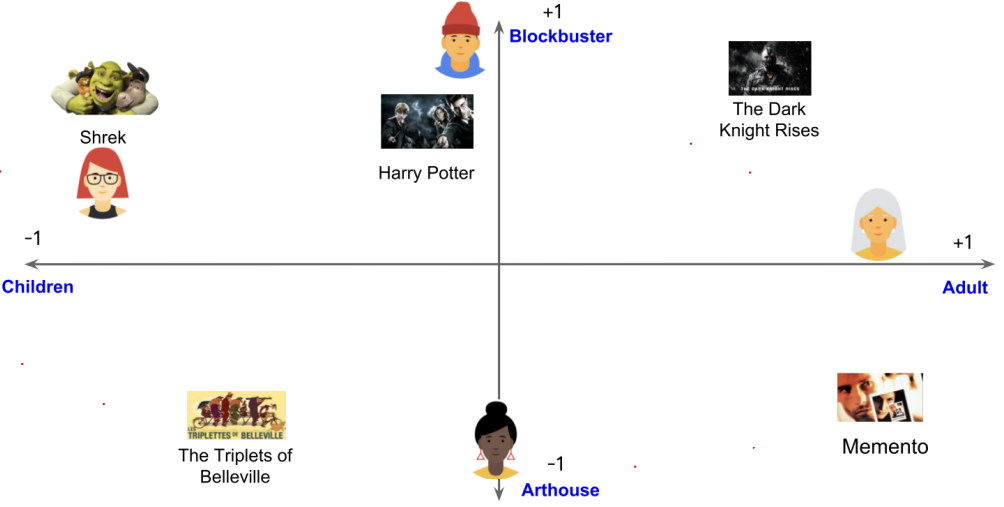
\includegraphics[width=0.8\linewidth]{images/img_20261023_182350.png}
\end{center}

Formally:
\begin{itemize}
    \item user feature vector $\theta^* \in \R^d$;
    \item item feature vector $a \in \R^d$;
    \item \textbf{utility}: $\sum_{i=1}^d a_i \theta_i = a^\top \theta$, i.e.\ the sum over features of (feature $a_i$ of the item) $\times$ (user's preference for feature $i$);
    \item \textbf{reward}: $a^\top\theta + \eta$, or more generally $g(a^\top\theta) + \eta$ for some function $g$. The reward is a \textbf{noisy signal of the utility}. It can be:
    \begin{itemize}
        \item continuous: watch time;
        \item discrete: rating given to the movie;
        \item binary: watched / not watched.
    \end{itemize}
\end{itemize}

\subsection{Modeling assumptions}

\begin{enumerate}
    \item \textbf{Both features $a$ and $\theta$ unknown}: collaborative filtering, matrix factorization.
    \begin{itemize}
        \item Identify similar users and similar items; use the preferences of similar users to recommend new items.
        \item Advantage: no need to handcraft features (they are learned).
        \item \textbf{Cold start problem}: each new user needs to rate a few items to get good recommendations; analogously for new items.
    \end{itemize}
    \item \textbf{Only the user features $\theta$ unknown} (item features $a$ known): this is the setting of this lecture.
    \begin{itemize}
        \item Recommend diverse movies to start with.
        \item With little data, we can already identify preferences: likes comedy, dislikes action, \dots
        \item Use the data to learn the user features.
    \end{itemize}
\end{enumerate}

\subsection{Recommender systems as bandits}

Suppose a new user signs up on Netflix.
\begin{itemize}
    \item Goal: recommend the best movies for this user over time, i.e.\ maximise the cumulative reward $\Leftrightarrow$ minimise the cumulative regret.
    \item Subgoal: learn the user preferences. We need to try out different movies, at the cost of showing a few bad movies.
    \item \textbf{Like multi-armed bandits}: it is an online learning problem with an exploration-exploitation tradeoff.
    \item \textbf{Unlike multi-armed bandits}: the reward from one arm (recommending a movie) gives information about the other arms!
\end{itemize}

\section{The linear bandit model}

\subsection{Definition}

\begin{definition}[Linear bandit]
\begin{itemize}
    \item Arms are represented as a set of vectors $\mathcal{A} = \{a_1, a_2, \dots, a_k\}$, $a_i \in \R^d$.
    \item Arm played at time $t$: $A_t \in \mathcal{A}$.
    \item Reward at time $t$:
    \[
    X_t = A_t^\top \theta^* + \eta_t = \langle \theta^*, A_t \rangle + \eta_t.
    \]
    \item Unknown parameter to be estimated: $\theta^* \in \R^d$.
    \item Noise model: the $\eta_t$ are independent for all $t$ and $\sigma$-subgaussian (we will mostly take $\sigma = 1$).
    \item Best arm: $a^* = \arg\max_{a\in\mathcal{A}} a^\top\theta^*$.
    \item Instantaneous regret:
    \[
    r_t = {a^*}^\top\theta^* - A_t^\top\theta^* = (a^* - A_t)^\top\theta^*.
    \]
\end{itemize}
\end{definition}

The key difference with the unstructured bandit: the $k$ unknown means $\mu_i = a_i^\top\theta^*$ are all determined by only $d$ unknown numbers (the entries of $\theta^*$). Observing $X_t$ for arm $A_t$ gives information about $\theta^*$ in the direction of $A_t$, hence about \emph{every} arm that is not orthogonal to $A_t$.

\begin{remark}[Reduction to the multi-armed bandit]
Linear bandits generalise unstructured bandits. Take $d = k$ and let the arms form an orthonormal basis, $a_i = e_i = (0, \dots, 0, 1, 0, \dots, 0)$ (a $1$ in position $i$). Then
\[
X_t = a_i^\top\theta^* + \eta_t = \theta_i^* + \eta_t,
\]
so $\theta_i^*$ plays the role of $\mu_i$, and pulling arm $i$ tells nothing about the other coordinates: we recover the standard $k$-armed bandit.
\end{remark}

\subsection{Flexibility of the linear bandit model}

\begin{itemize}
    \item The vector $\theta$ can include \textbf{known aspects of the user context}: age, gender, region, \dots; explicitly mentioned interests; behavioural statistics (number of comedy movies watched), etc.
    \item The \textbf{action set} $\mathcal{A}_t = \{a_1^t, a_2^t, \dots, a_k^t\}$ \textbf{can vary with time}, e.g.:
    \begin{itemize}
        \item the same user's context can change (restaurants in a new city; recommending among some search results; \dots);
        \item different users at different times;
        \item new items appear, old ones disappear.
    \end{itemize}
    The linear bandit model extends easily to a time-varying, arbitrary action set $\mathcal{A}_t$ (this is sometimes called a \emph{contextual} linear bandit). In the unstructured setting, a brand new arm would have to be explored from scratch; here, its feature vector immediately gives an estimate of its reward.
    \item \textbf{Interpreting $\theta^*$}: a \textbf{global weight vector over features}, and the expected reward of $A_t$ is $A_t^\top\theta^*$. For instance, if the feature vector contains a crossed feature (young user, animation movie), a positive $\theta_i^*$ for this feature means that young people prefer animation movies.
\end{itemize}

\subsection{Formulations of regret for linear bandits}

\begin{itemize}
    \item Instantaneous regret: $r_t = {a^*}^\top\theta^* - A_t^\top\theta^* = (a^* - A_t)^\top\theta^*$. Note that it \textbf{does not depend on the noise} $\eta_t$.
    \item \textbf{Random cumulative regret}:
    \[
    \hat{R}_n(A_1, \dots, A_n) = \sum_{t=1}^n \Big( \max_{a\in\mathcal{A}_t} \langle\theta^*, a\rangle - \langle\theta^*, A_t\rangle \Big) = \sum_{t=1}^n r_t.
    \]
    It is a random variable: it depends on the (random) choice of actions.
    \item \textbf{Regret}:
    \[
    R_n = \mathbb{E}\big[\hat{R}_n\big] = \mathbb{E}\left[\sum_{t=1}^n \max_{a\in\mathcal{A}_t}\langle\theta^*, a\rangle - \sum_{t=1}^n X_t\right].
    \]
    Taking the expectation marginalises out the choice of actions. The two expressions coincide since $\mathbb{E}[X_t \mid A_t] = \langle\theta^*, A_t\rangle$ (the noise has zero mean).
\end{itemize}

\begin{remark}
The analysis of LinUCB will first bound $\hat{R}_n$ \emph{with high probability} (on a good event), and then convert it into a bound on $R_n$. This is the same ``good event / bad event'' strategy as for UCB.
\end{remark}

\section{Estimating $\theta^*$ via linear regression}

\subsection{Least squares}

\begin{itemize}
    \item Data: $(A_1, X_1, A_2, X_2, \dots, A_t, X_t)$.
    \item Model: $X_s = A_s^\top\theta^* + \eta_s$, with $\theta^* \in \R^d$ unknown, to be estimated, and $\eta_s \in \R$ a $1$-subgaussian random variable.
    \item This is exactly \textbf{linear regression}. The least squares problem is
    \[
    \min_\theta \sum_{s\in[t]} \big(X_s - A_s^\top\theta\big)^2.
    \]
\end{itemize}

\begin{definition}[Least squares estimator, design matrix]
\[
\hat{\theta}_t = V_t^{-1}\sum_{s\in[t]} A_s X_s, \qquad V_t = \sum_{s\in[t]} A_s A_s^\top \in \R^{d\times d}.
\]
$V_t$ is called the \textbf{design matrix}: it summarises which directions have been explored. It is symmetric and positive semi-definite.
\end{definition}

\begin{proof}[Derivation]
The objective $L(\theta) = \sum_s (X_s - A_s^\top\theta)^2$ is convex in $\theta$, with gradient
\[
\nabla L(\theta) = -2\sum_s A_s\big(X_s - A_s^\top\theta\big).
\]
Setting it to zero gives the normal equations $\big(\sum_s A_sA_s^\top\big)\theta = \sum_s A_s X_s$, i.e.\ $V_t\theta = \sum_s A_s X_s$, hence $\hat{\theta}_t = V_t^{-1}\sum_s A_s X_s$ when $V_t$ is invertible.
\end{proof}

\begin{center}
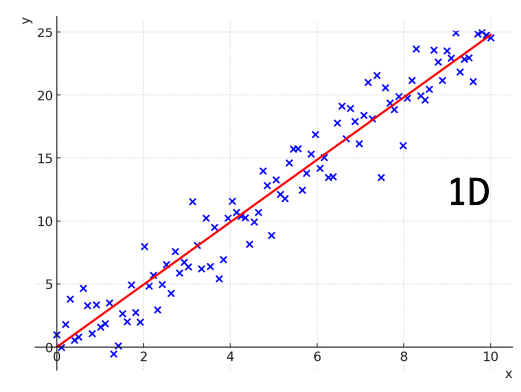
\includegraphics[width=0.3\linewidth]{images/img_20261024_132333.png}
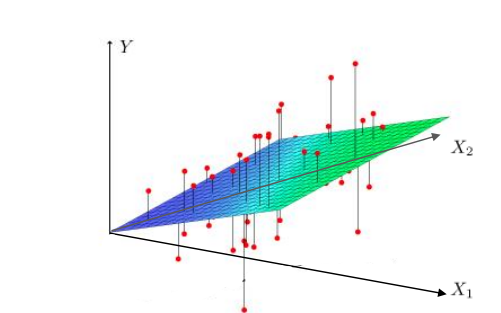
\includegraphics[width=0.4\linewidth]{images/img_20261024_132346.png}
\end{center}

\subsection{The estimator is unbiased}

Substituting the model $X_s = A_s^\top\theta^* + \eta_s$ (and treating the $A_s$ as fixed):
\[
\hat{\theta}_t = V_t^{-1}\sum_{s\in[t]} A_s\big(A_s^\top\theta^* + \eta_s\big) = \underbrace{V_t^{-1} V_t}_{=I}\,\theta^* + V_t^{-1}\sum_{s\in[t]} A_s\eta_s = \theta^* + V_t^{-1}\sum_{s\in[t]} A_s\eta_s,
\]
so, since $\mathbb{E}[\eta_s] = 0$,
\[
\mathbb{E}\big[\hat{\theta}_t\big] = \mathbb{E}\left[V_t^{-1}\sum_{s\in[t]}\big(A_sA_s^\top\theta^* + A_s\eta_s\big)\right] = \theta^*.
\]
Moreover, if the noise has variance $\sigma^2$, the covariance of the estimator is
\[
\text{Cov}\big(\hat{\theta}_t\big) = V_t^{-1}\left(\sum_s A_sA_s^\top \sigma^2\right)V_t^{-1} = \sigma^2 V_t^{-1}.
\]
This is the key fact: \textbf{the uncertainty of $\hat{\theta}_t$ is quantified by $V_t^{-1}$}.

\subsection{Uncertainty in linear regression: 1D case}

In 1D, $\theta^*$ and $\hat{\theta}$ are scalars: $\hat{\theta}_t = \frac{\sum_s A_sX_s}{\sum_s A_s^2}$ and $\text{Var}(\hat{\theta}_t) = \frac{\sigma^2}{\sum_s A_s^2}$. The uncertainty in $\hat{\theta}$ can be conveyed through \textbf{confidence intervals}:
\begin{itemize}
    \item more noise in the data $\Rightarrow$ larger confidence intervals;
    \item more data points $\Rightarrow$ smaller confidence intervals (the width is proportional to $\sigma/\sqrt{\sum_s A_s^2}$).
\end{itemize}

\subsection{Uncertainty in linear regression: 2D case}

In dimension $d \geq 2$, confidence intervals become \textbf{confidence ellipses} (ellipsoids) $\mathcal{C}_t$ centred at $\hat{\theta}_t$.

\begin{center}
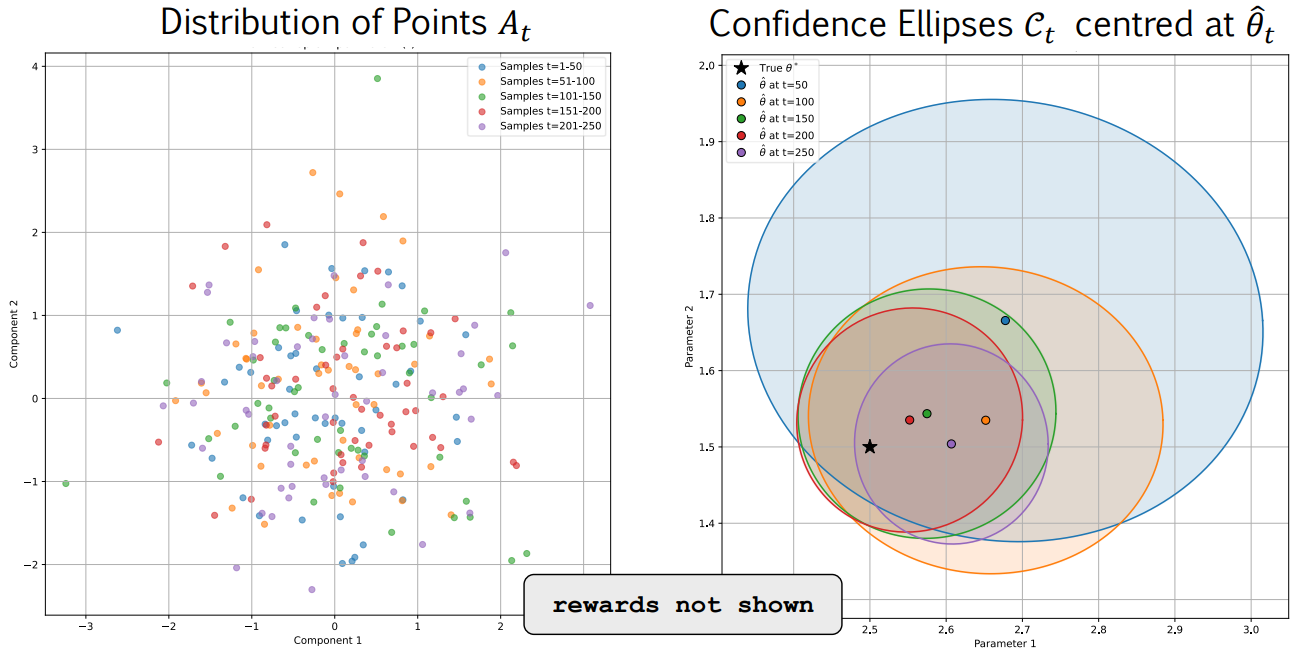
\includegraphics[width=0.8\linewidth]{images/img_20261024_135846.png}
\end{center}

The directions that have been better explored (many data points $A_s$ along them) have less uncertainty (the ellipse is narrow in those directions); the less explored directions have more uncertainty (the ellipse is elongated).

\subsection{Why ellipses?}

\begin{itemize}
    \item The collection of data points is represented by the design matrix $V_t = \sum_{s\in[t]} A_sA_s^\top$.
    \item More data points in a certain direction $a$ $\Rightarrow$ the eigenvalues of $V_t$ are larger in that direction ($a^\top V_t a = \sum_s \langle a, A_s\rangle^2$ grows).
    \item More data points in a certain direction $a$ $\Rightarrow$ better estimate of the component of $\theta^*$ parallel to $a$.
    \item The uncertainty of $\theta^*$ is quantified by $V_t^{-1}$ $\Rightarrow$ more uncertainty along the larger eigenvalues of $V_t^{-1}$ (i.e.\ the smaller eigenvalues of $V_t$).
\end{itemize}

\begin{definition}[Weighted norm, confidence set]
For a positive definite matrix $V$, define the norm $\|x\|_V = \sqrt{x^\top V x}$. The confidence sets are
\[
\mathcal{C}_t = \Big\{\theta \in \R^d : \big\|\theta - \hat{\theta}_{t-1}\big\|_{V_{t-1}}^2 \leq \beta_t\Big\},
\]
where $\beta_t$ is a radius chosen so that $\theta^* \in \mathcal{C}_t$ with high probability.
\end{definition}

\begin{remark}[Geometry]
Write $V = \sum_j \lambda_j u_ju_j^\top$ (eigendecomposition). Then $\|\theta - \hat{\theta}\|_V^2 = \sum_j \lambda_j \langle \theta - \hat{\theta}, u_j\rangle^2 \leq \beta$ is an ellipsoid whose axes are the eigenvectors $u_j$, with semi-axis lengths $\sqrt{\beta/\lambda_j}$. A large eigenvalue (well-explored direction) gives a short axis (little uncertainty), a small eigenvalue gives a long axis. In 1D, this reduces to the interval $|\theta - \hat{\theta}| \leq \sqrt{\beta/\sum_s A_s^2}$.
\end{remark}

\subsection{Regularisation}

\textbf{What if $V_t$ is not invertible?} This happens for instance at the beginning ($t < d$), or whenever the played arms do not span $\R^d$: some directions have never been explored, and the least squares problem has infinitely many solutions.

\textbf{Simple fix}: use a regulariser (ridge regression). Solve
\[
\min_\theta \sum_{s\in[t]}\big(X_s - A_s^\top\theta\big)^2 + \lambda\|\theta\|_2^2,
\]
whose solution is (same derivation, with the extra gradient term $2\lambda\theta$)
\[
\hat{\theta}_t = V_t^{-1}\sum_{s\in[t]} A_sX_s, \qquad V_t = \lambda I + \sum_{s\in[t]} A_sA_s^\top.
\]
For $\lambda > 0$, $V_t$ is positive definite (all eigenvalues $\geq \lambda$), hence always invertible. The price is a small bias of $\hat{\theta}_t$ towards $0$, which vanishes as data accumulates.

\begin{center}
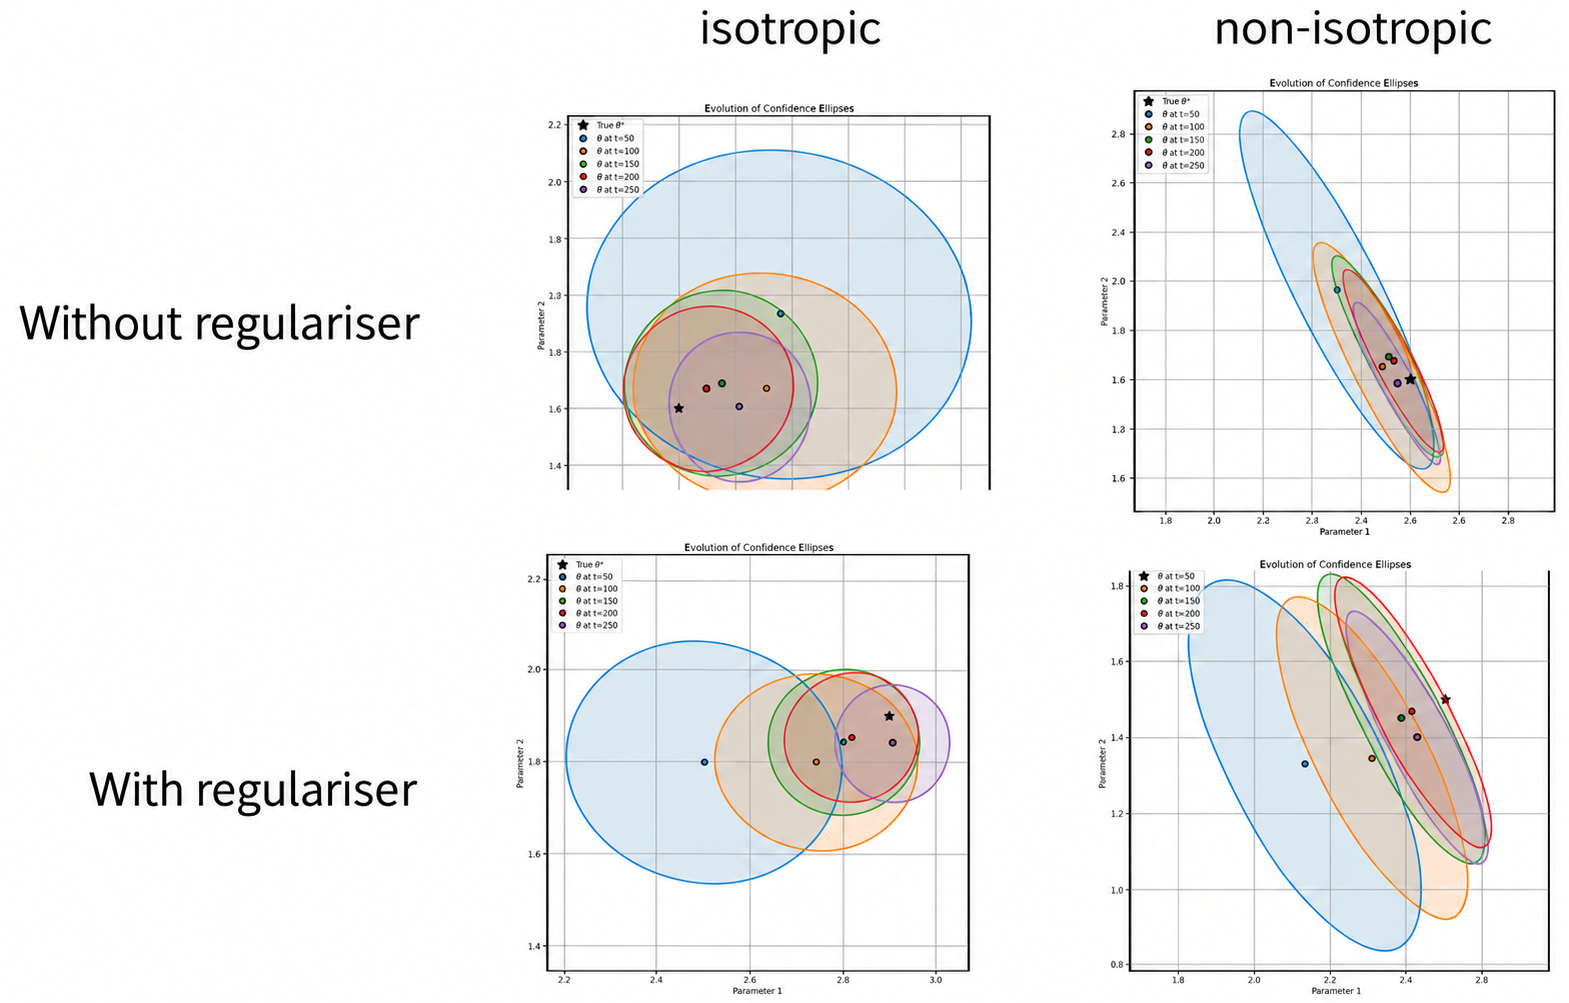
\includegraphics[width=\linewidth]{images/img_20261024_150338.png}
\end{center}

\textbf{Impact on the confidence ellipses}. Each panel shows the true $\theta^*$ (star), the estimates $\hat{\theta}_t$ for $t = 50, \dots, 250$ and the corresponding confidence ellipses. In all cases, the ellipses shrink over time and keep containing $\theta^*$.
\begin{itemize}
    \item \textbf{Isotropic vs non-isotropic} refers to the distribution of the played vectors $A_s$: if they are spread evenly in all directions, $V_t$ has similar eigenvalues and the confidence sets are nearly circles; if they are concentrated along one direction, the ellipses are narrow along that (well-explored) direction and elongated along the poorly explored one.
    \item \textbf{With a regulariser}, the estimate is biased towards $0$ (penalty $\lambda\|\theta\|_2^2$): early estimates are visibly pulled towards the origin, then move towards $\theta^*$ as data accumulates, since $\lambda I$ becomes negligible compared to $\sum_s A_sA_s^\top$. In exchange, $V_t$ is always invertible, and $V_0 = \lambda I$ makes the initial confidence set an isotropic ball.
\end{itemize}

\section{LinUCB: UCB for linear bandits}

\subsection{Algorithm}

\textbf{Notation}:
\begin{itemize}
    \item $V_0 = \lambda I$, \quad $V_t = \lambda I + \sum_{s\in[t]} A_sA_s^\top$;
    \item $\hat{\theta}_t = V_t^{-1}\sum_{s\in[t]} A_sX_s$;
    \item $\mathcal{C}_t = \big\{\theta \in \R^d : \|\theta - \hat{\theta}_{t-1}\|_{V_{t-1}}^2 \leq \beta_{t-1}\big\}$;
    \item $1 \leq \beta_1 \leq \beta_2 \leq \dots \leq \beta_n$ (non-decreasing radii).
\end{itemize}

The principle is \textbf{optimism in the face of uncertainty}: the UCB of an arm $a$ is the largest reward it could have under any parameter that is still plausible (i.e.\ in the confidence set).

\begin{definition}[LinUCB, abstract form]
\begin{tabbing}
\hspace{1.5em}\=\hspace{1.5em}\=\kill
\textbf{for} $t = 1, 2, \dots, n$ \textbf{do}: \\
\> \textbf{for} all arms $a \in \mathcal{A}_t$: compute $UCB_t(a) = \max_{\theta\in\mathcal{C}_t} a^\top\theta$; \\
\> play $A_t = \arg\max_{a\in\mathcal{A}_t} UCB_t(a)$; \\
\> observe $X_t$ and update $V_t$, $\hat{\theta}_t$, $\mathcal{C}_t$.
\end{tabbing}
\end{definition}

\begin{center}
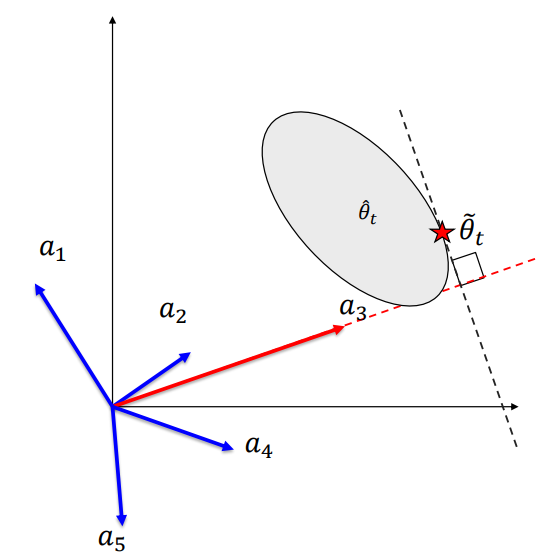
\includegraphics[width=0.4\linewidth]{images/img_20261024_151616.png}
\end{center}

\subsection{Computing the UCB}

Combining the two maximisations,
\[
A_t = \arg\max_{a\in\mathcal{A}_t} UCB_t(a), \quad UCB_t(a) = \max_{\theta\in\mathcal{C}_t} a^\top\theta
\quad\Rightarrow\quad
(A_t, \tilde{\theta}_t) = \arg\max_{(a,\theta)\in\mathcal{A}_t\times\mathcal{C}_t} a^\top\theta.
\]
So LinUCB jointly picks an arm $A_t$ and an \textbf{optimistic parameter} $\tilde{\theta}_t \in \mathcal{C}_t$ (the point of the ellipsoid that makes $A_t$ look best).

\begin{theorem}[Closed form of the UCB]
If $\mathcal{C}_t = \big\{\theta : \|\theta - \hat{\theta}_{t-1}\|_{V_{t-1}}^2 \leq \beta_t\big\}$, then
\[
UCB_t(a) = \max_{\theta\in\mathcal{C}_t} a^\top\theta = \underbrace{a^\top\hat{\theta}_{t-1}}_{\text{exploitation}} + \underbrace{\sqrt{\beta_t}\,\|a\|_{V_{t-1}^{-1}}}_{\text{optimistic bonus}}.
\]
\end{theorem}

\begin{definition}[LinUCB, explicit form]
\begin{tabbing}
\hspace{1.5em}\=\kill
\textbf{for} $t = 1, 2, \dots, n$ \textbf{do}: \\
\> play $A_t = \arg\max_{a\in\mathcal{A}_t}\left( a^\top\hat{\theta}_{t-1} + \sqrt{\beta_t}\,\|a\|_{V_{t-1}^{-1}} \right)$; \\
\> observe $X_t$ and update $V_t$, $\hat{\theta}_t$, $\mathcal{C}_t$.
\end{tabbing}
\end{definition}

\subsection{LinUCB in practice}

Setting: linear bandit with $k = 100$ arms and $d = 5$ dimensional features.

\begin{center}
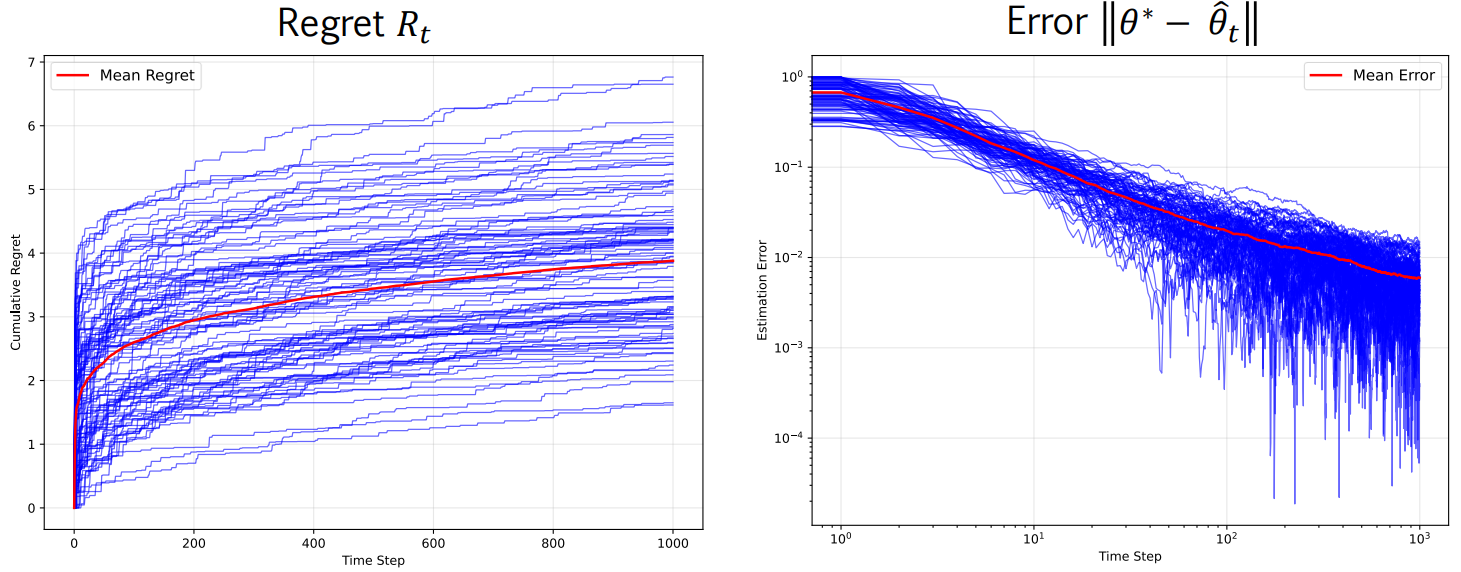
\includegraphics[width=0.8\linewidth]{images/img_20261024_152606.png}
\end{center}

\begin{itemize}
    \item \textbf{Regret} $R_t = O(\sqrt{t})$ (up to log factors), similar to unstructured bandits (problem-independent rate).
    \item \textbf{Error} $\|\theta^* - \hat{\theta}_t\| = O(1/\sqrt{t})$, similar to linear regression.
\end{itemize}

\begin{center}
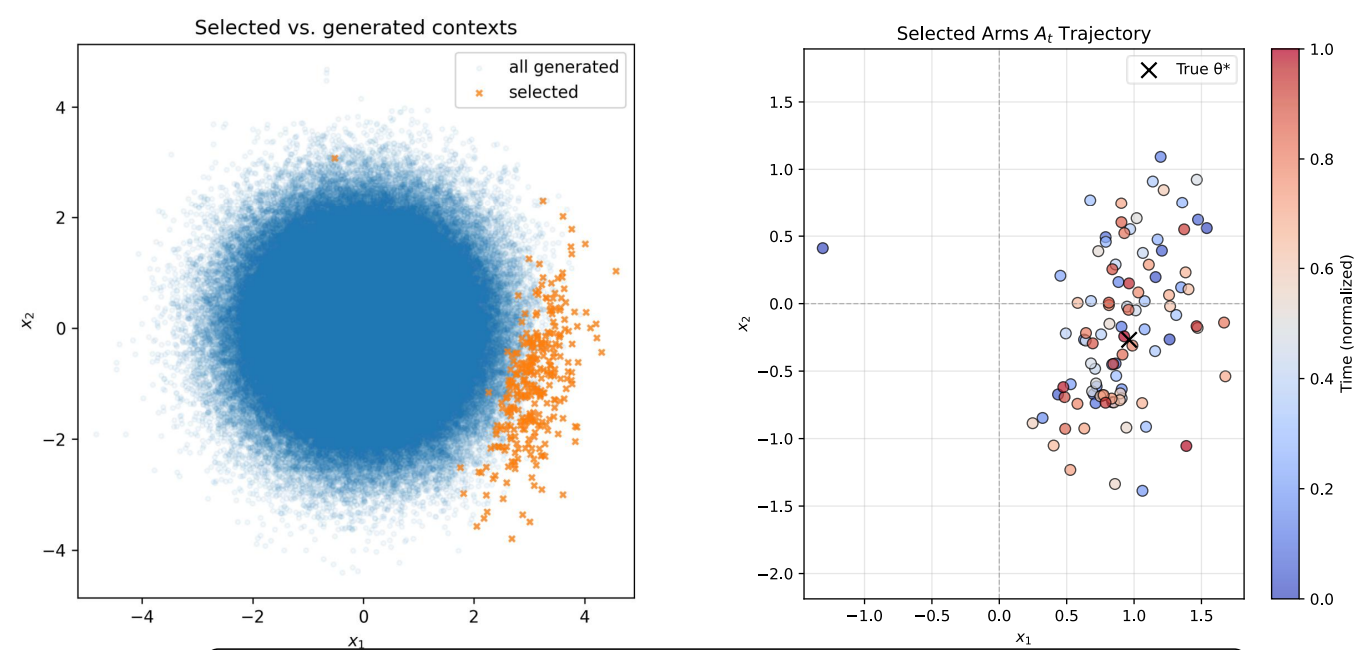
\includegraphics[width=0.8\linewidth]{images/img_20261024_152732.png}
\end{center}

\textbf{Actions over time}: the selected arms align in the direction of $\theta^*$ (the best arms are those with the largest projection on $\theta^*$). Consequently, $\theta^*$ is estimated precisely in that direction, and less precisely in the orthogonal directions: this is enough, since precision is only needed to rank the near-optimal arms.

\begin{center}
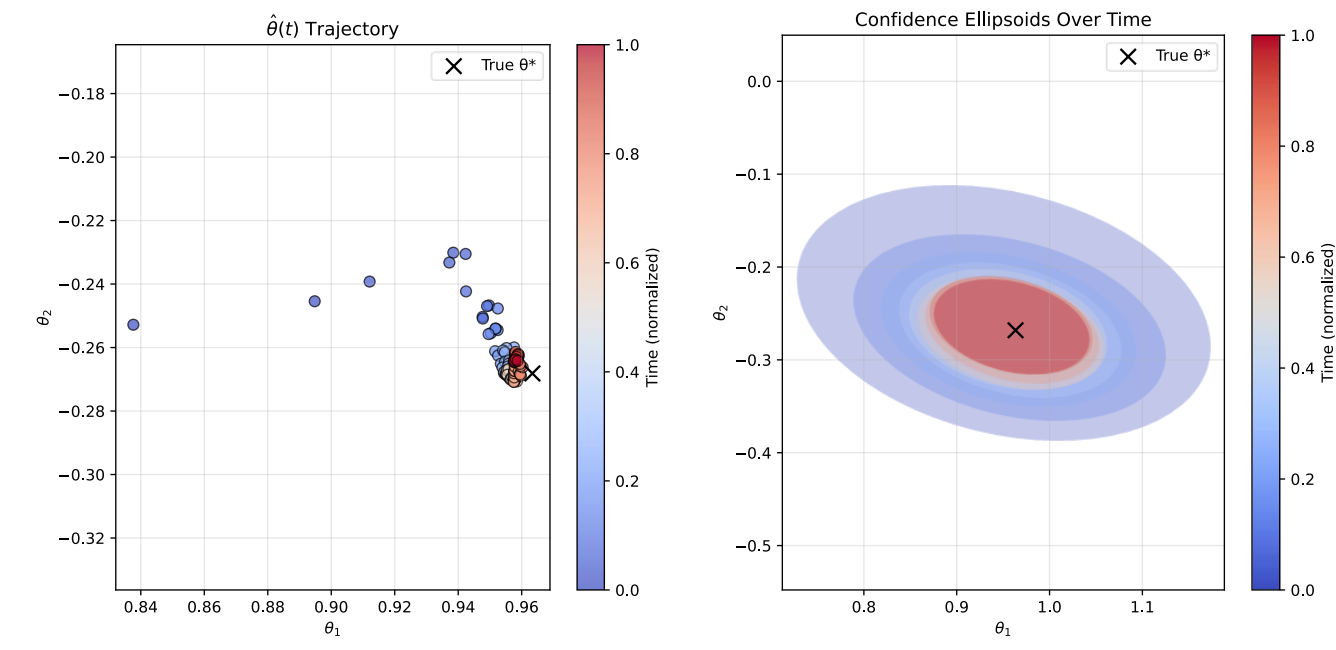
\includegraphics[width=0.8\linewidth]{images/img_20261024_152929.png}
\end{center}

\textbf{Confidence ellipsoids with time}: they shrink around $\theta^*$, faster in the directions that are played often.

\section{Analysis of LinUCB}

\subsection{High-level view}
\begin{center}  
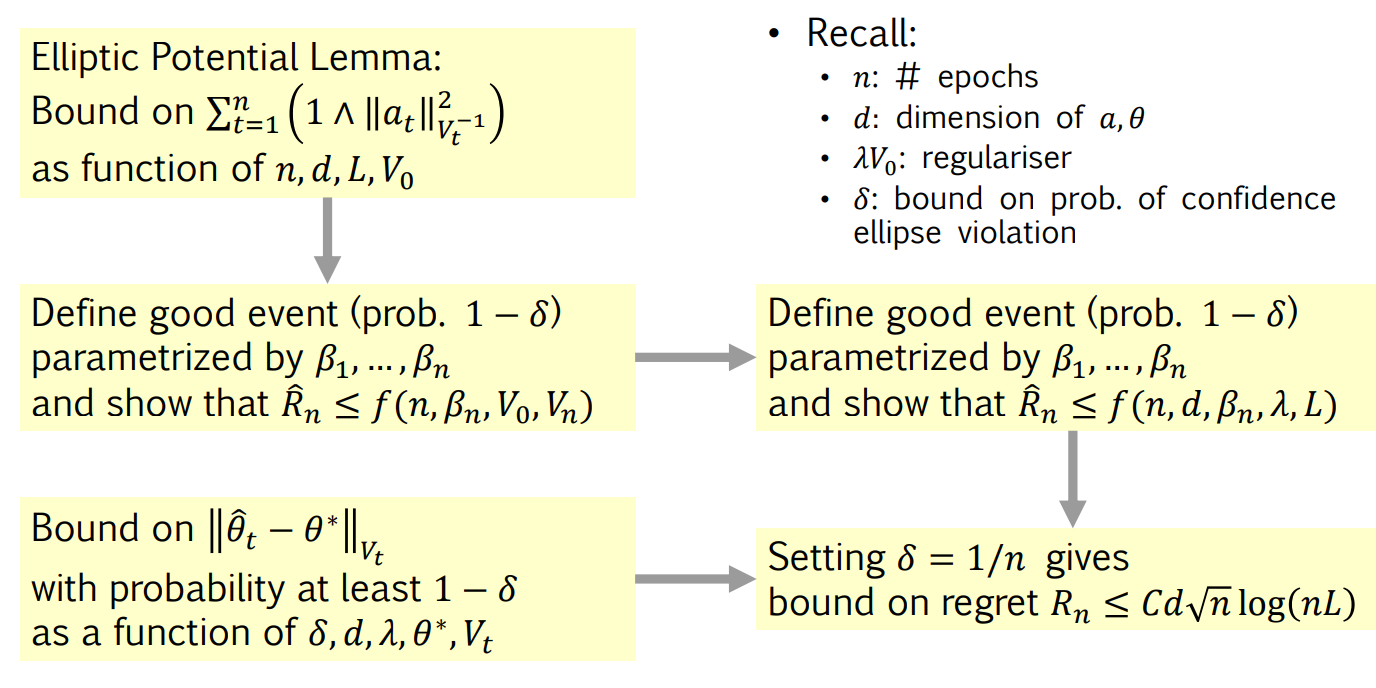
\includegraphics[width=0.7\linewidth]{images/img_20261024_154619.png}
\end{center}

\subsection{Intuition for the concentration bound (single arm)}

We first prove a simple concentration inequality for a single, fixed arm $a$ (with $\lambda = 0$, and treating the $A_s$ as fixed).

Recall $\hat{\theta}_t = V_t^{-1}\sum_{s\in[t]} A_sX_s$ and $X_s = A_s^\top\theta^* + \eta_s$. Then
\[
\big\langle a, \hat{\theta}_t - \theta^*\big\rangle = \left\langle a, V_t^{-1}\sum_{s\in[t]} A_s\big(A_s^\top\theta^* + \eta_s\big) - \theta^*\right\rangle.
\]
Observe that $\sum_s A_sA_s^\top\theta^* = V_t\theta^*$, so $V_t^{-1}\sum_s A_sA_s^\top\theta^* = \theta^*$. Hence
\[
\big\langle a, \hat{\theta}_t - \theta^*\big\rangle = \left\langle a, V_t^{-1}\sum_{s\in[t]} A_s\eta_s\right\rangle = \sum_{s\in[t]} \big\langle a, V_t^{-1}A_s\big\rangle\,\eta_s.
\]
This is a \textbf{linear combination of independent, $1$-subgaussian random variables} $(\eta_s)_{s\in[t]}$. Recall the properties of subgaussian random variables:
\begin{itemize}
    \item $\eta$ is $1$-subgaussian $\Rightarrow$ $\alpha\eta$ is $|\alpha|$-subgaussian;
    \item $\eta_1, \eta_2$ independent, $\sigma_1$- and $\sigma_2$-subgaussian $\Rightarrow$ $\eta_1 + \eta_2$ is $\sqrt{\sigma_1^2 + \sigma_2^2}$-subgaussian.
\end{itemize}
Therefore $\sum_s \langle a, V_t^{-1}A_s\rangle\eta_s$ is subgaussian, with variance proxy
\[
\sum_{s\in[t]}\big\langle a, V_t^{-1}A_s\big\rangle^2 = a^\top V_t^{-1}\left(\sum_{s\in[t]} A_sA_s^\top\right)V_t^{-1}a = a^\top V_t^{-1}V_tV_t^{-1}a = a^\top V_t^{-1}a = \|a\|_{V_t^{-1}}^2.
\]
Applying the concentration inequality for subgaussians ($\mathbb{P}(Z \geq \sqrt{2\sigma^2\ln(1/\delta)}) \leq \delta$ for $Z$ $\sigma$-subgaussian):
\[
\mathbb{P}\left(\big\langle a, \hat{\theta}_t - \theta^*\big\rangle \geq \sqrt{2\|a\|_{V_t^{-1}}^2\ln(1/\delta)}\right) \leq \delta.
\]
This is the exact analogue of the UCB confidence interval: $a^\top\hat{\theta}_t$ estimates $a^\top\theta^*$ with an error of order $\|a\|_{V_t^{-1}}\sqrt{2\ln(1/\delta)}$, and in the MAB case $\|e_i\|_{V_t^{-1}}^2 = 1/T_i(t)$.

\subsection{The simple bound is not sufficient}

The bound above
\[
\mathbb{P}\left(\big\langle a, \hat{\theta}_t - \theta^*\big\rangle \geq \sqrt{2\ln(1/\delta)\sum_{s\in[t]}\big\langle a, V_t^{-1}A_s\big\rangle^2}\right) \leq \delta
\]
holds only for a \textbf{single arm}. For regret guarantees, we need such a bound for \textbf{all arms} simultaneously.
\begin{itemize}
    \item One option: a union bound over all $k$ arms. If the action set $\mathcal{A} = \{a_1, \dots, a_k\}$ is small, this is a reasonable strategy, and the regret bound will scale with $\log k$.
    \item For large (or infinite, or time-varying) action sets, we want a bound \textbf{independent of $k$}. We then need a bound on $\mathbb{P}\big(\|\hat{\theta}_t - \theta^*\|_{V_t} \geq \beta_t\big)$ instead of on $\langle a, \hat{\theta}_t - \theta^*\rangle$: a bound on the whole vector, valid for all directions at once.
    \item Moreover, in a bandit, $A_s$ depends on past observations (hence on the past noise), so the $A_s$ are not fixed and the argument above is not rigorous as such. See L\&S, Chapter 20.
\end{itemize}

\subsection{Key concentration result}

\begin{theorem}[Theorem 20.5 in L\&S, not proven in class]
Suppose we have a sequence of data points $(A_1, X_1, A_2, X_2, \dots)$ satisfying
\begin{itemize}
    \item $X_t = \langle\theta^*, A_t\rangle + \eta_t$, with $\eta_t$ independent and $1$-subgaussian;
    \item each $A_t$ may depend on the past $(A_1, X_1, \dots, A_{t-1}, X_{t-1})$ (any bandit algorithm).
\end{itemize}
Let $\hat{\theta}_t$ be the least-squares estimator with regulariser weight $\lambda$. Fix $\delta \in (0,1)$. Then, with probability at least $1 - \delta$, it holds \textbf{for all} $t \in \mathbb{N}$:
\[
\big\|\hat{\theta}_t - \theta^*\big\|_{V_t} < \sqrt{\lambda}\,\|\theta^*\|_2 + \sqrt{2\ln\frac{1}{\delta} + \ln\frac{\det V_t}{\lambda^d}}.
\]
\end{theorem}

\subsection{Understanding the good event}

\begin{itemize}
    \item Good event: $\forall t$, $\theta^* \in \mathcal{C}_t = \big\{\theta \in \R^d : \|\theta - \hat{\theta}_{t-1}\|_{V_{t-1}}^2 \leq \beta_t\big\}$.
    \item It holds with probability $1 - \delta$ (by the theorem above, for a suitable $\beta_t$).
    \item Intuitively:
    \begin{itemize}
        \item $\|\theta^* - \hat{\theta}_{t-1}\|_{V_{t-1}}^2 \leq \beta_t$ is a concentration event, and needs $\beta_t = O(\log t)$;
        \item we expect the eigenvalues of $V_{t-1}$ to grow proportionally to $t-1$ (if all directions keep being explored);
        \item since $\|x\|_2^2 \leq \|x\|_V^2/\lambda_{\min}(V)$, put together we get
        \[
        \big\|\theta^* - \hat{\theta}_t\big\|_2 = O\left(\sqrt{\frac{\log t}{t}}\right).
        \]
    \end{itemize}
    \item With more data, the estimate $\hat{\theta}_t$ gets closer to $\theta^*$.
\end{itemize}

\subsection{Regret guarantees for LinUCB}

\begin{theorem}[Regret of LinUCB]
Assume that:
\begin{itemize}
    \item rewards are bounded: $\max_{t\in[n]}\sup_{a,b\in\mathcal{A}_t} (a - b)^\top\theta^* \leq 1$;
    \item arm features are bounded: $\|a\|_2 \leq L$ for all $a \in \bigcup_{t=1}^n \mathcal{A}_t$;
    \item $\beta_1, \beta_2, \dots$ are chosen such that, with probability $\geq 1-\delta$ where $\delta = 1/n$,
    \[
    \forall t, \quad \theta^* \in \mathcal{C}_t = \big\{\theta\in\R^d : \|\theta - \hat{\theta}_{t-1}\|_{V_{t-1}}^2 \leq \beta_t\big\};
    \]
    \item $\beta_t = O\left(\ln\frac1\delta + d\ln\frac{d\lambda + nL^2}{d\lambda}\right)$ suffices.
\end{itemize}
Then
\[
R_n = O\big(d\sqrt{n}\,\log(nL)\big).
\]
\end{theorem}

\begin{remark}
\begin{itemize}
    \item The bound is \textbf{independent of the number of arms $k$}! It depends on the dimension $d$ instead. The information structure (pulling one arm informs about the others) is what makes this possible.
    \item Compare with the unstructured bound $O(\sqrt{kn\ln n})$: for $k \gg d^2$ (many arms, few features), linear bandits are much better. In the MAB reduction ($d = k$), this bound gives $O(k\sqrt{n}\log n)$, which is worse than $O(\sqrt{kn\log n})$ by a $\sqrt{k}$ factor: the price of a general analysis that does not exploit the orthogonality of the arms.
    \item The rate in $n$ is $\sqrt{n}$ (up to logs), as for the problem-independent bound of UCB.
\end{itemize}
\end{remark}

\subsection{Regret: variation with $k$ and $d$}

Setting: linear bandit with arm features $a_i^t \sim \mathcal{N}(0, I_d)$.

\begin{center}
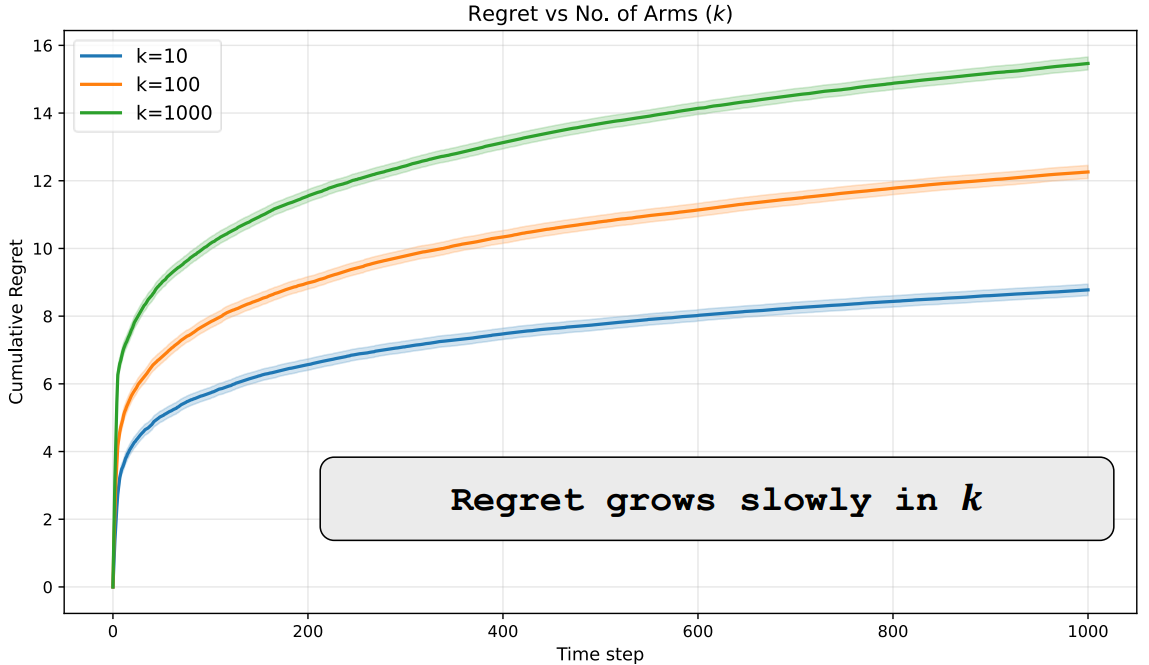
\includegraphics[width=0.6\linewidth]{images/img_20261024_153716.png}
\end{center}

\textbf{Variation with $k$} ($d = 5$): the regret \textbf{grows slowly in $k$}. (More arms mean the best arm is a bit better aligned with $\theta^*$, but no extra exploration per arm is needed.)

\begin{center}
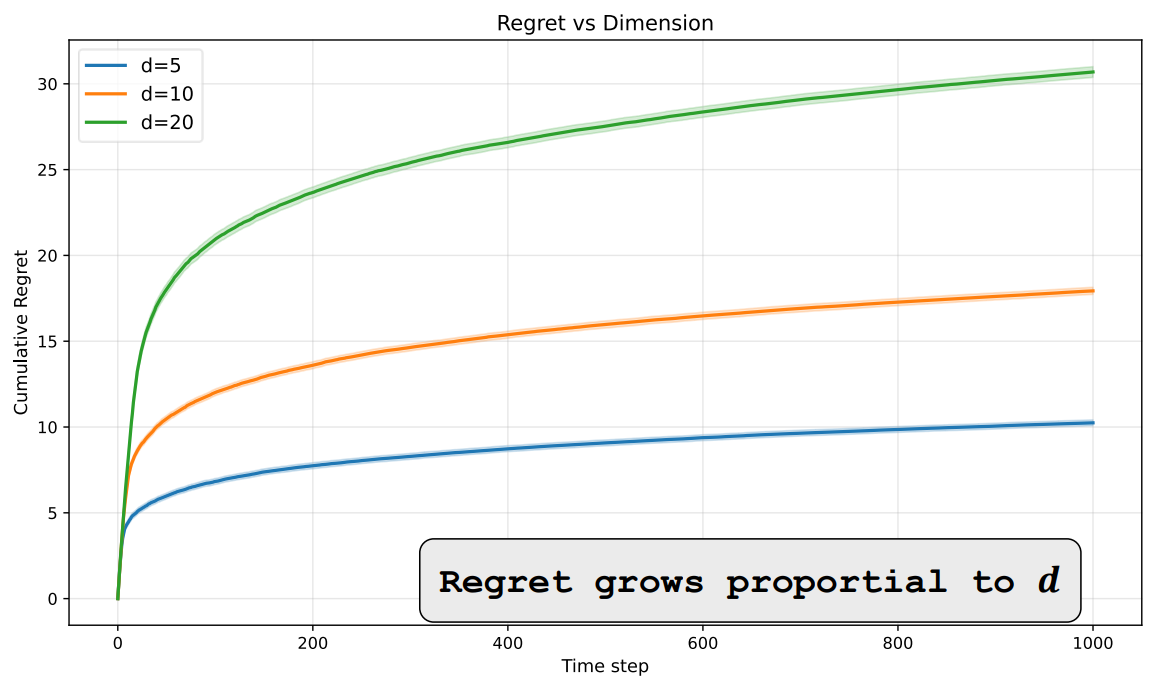
\includegraphics[width=0.6\linewidth]{images/img_20261024_153819.png}
\end{center}

\textbf{Variation with $d$} ($k = 100$): the regret \textbf{grows proportionally to $d$}, as predicted by the bound.

\section{Thompson Sampling for linear bandits}

Key ideas in Thompson Sampling:
\begin{itemize}
    \item maintain a belief distribution over the unknown parameters;
    \item at each time $t$: sample parameters from the belief distribution (exploration), then play assuming that the sample is the true parameter (exploitation).
\end{itemize}

In linear bandits, the unknown parameter is $\theta^*$:
\begin{itemize}
    \item maintain a \textbf{multivariate Gaussian belief} $f_t(\theta^*) \sim \mathcal{N}(\mu_t, \Sigma_t)$;
    \item after sampling $\tilde{\theta}_t \sim f_t$, play
    \[
    A_t = \arg\max_{a\in\mathcal{A}_t} a^\top\tilde{\theta}_t;
    \]
    \item this is \textbf{computationally faster} than LinUCB's $A_t = \arg\max_{a\in\mathcal{A}_t}\big(a^\top\hat{\theta}_{t-1} + \sqrt{\beta_t}\|a\|_{V_{t-1}^{-1}}\big)$
    \item heuristic choice of the belief:
    \[
    \mu_t = \hat{\theta}_t = V_t^{-1}\sum_{s\in[t]} A_sX_s, \qquad \Sigma_t^{-1} = V_t = \sum_{s\in[t]} A_sA_s^\top \;\;(+\lambda I).
    \]
\end{itemize}

\section{Generalised linear bandits}

\begin{itemize}
    \item Linear bandit reward model: $X_t = A_t^\top\theta^* + \eta_t$.
    \begin{itemize}
        \item The reward can be unbounded.
        \item Unrealistic for scenarios where the reward is binary: click or no click.
    \end{itemize}
    \item Better model:
    \[
    X_t = g\big(A_t^\top\theta^*\big) + \eta_t,
    \]
    where $g : \R \to [0,1]$ is a nonlinear \textbf{link function}, e.g.\ the sigmoid $g(z) = \frac{1}{1 + e^{-z}}$.
    \item This captures: $X_t = 1$ with probability $g(A_t^\top\theta^*)$, $X_t = 0$ otherwise.
    \item Often used in practice, e.g.\ online advertisement placement (click-through rates).
    \item All principles of LinUCB and Thompson Sampling carry over! The only change: $\hat{\theta}_t$ is estimated by \textbf{logistic regression} (maximum likelihood) instead of least squares. Since $g$ is increasing, the best arm is still $\arg\max_a a^\top\theta^*$.
    \item Tight regret bounds have only been discovered recently (2020 onwards).
\end{itemize}

\section{Summary}

\begin{itemize}
    \item \textbf{Linear bandit model}: arms have known feature vectors $a \in \R^d$, and the reward is a noisy linear function of the features, $X_t = A_t^\top\theta^* + \eta_t$, with $\theta^* \in \R^d$ unknown. Model for recommender systems (item features $a$, user preferences $\theta^*$). The action set $\mathcal{A}_t$ can change over time. The MAB is the special case $a_i = e_i$.
    \item \textbf{Different information structure}: the unknown is $\theta^* \in \R^d$, and pulling one arm conveys information about the rewards of the other arms. Regret scales as $O(d\sqrt{n})$ (up to logs) rather than $O(\sqrt{kn})$.
    \item \textbf{Parameter estimation by linear regression}: $\hat{\theta}_t = V_t^{-1}\sum_s A_sX_s$, unbiased (without regulariser), with covariance $V_t^{-1}$. Importance of the regulariser: $V_t = \lambda I + \sum_s A_sA_s^\top$ is always invertible, and the initial confidence set is an isotropic ball.
    \item \textbf{Uncertainty} in the estimate is quantified by $V_t = \sum_s A_sA_s^\top$: uncertainty intervals become \textbf{uncertainty ellipsoids} $\mathcal{C}_t = \{\theta : \|\theta - \hat{\theta}_{t-1}\|_{V_{t-1}}^2 \leq \beta_t\}$, narrow in well-explored directions.
    \item \textbf{LinUCB}: extends the optimism in the face of uncertainty principle: $A_t = \arg\max_a \max_{\theta\in\mathcal{C}_t} a^\top\theta = \arg\max_a\big(a^\top\hat{\theta}_{t-1} + \sqrt{\beta_t}\|a\|_{V_{t-1}^{-1}}\big)$. Provable regret guarantee $R_n = O(d\sqrt{n}\log(nL))$; key point: \textbf{independent of $k$}. Analysis: concentration of $\|\hat{\theta}_t - \theta^*\|_{V_t}$ uniformly in $t$ (L\&S Thm 20.5, with $\beta_t = O(\log\frac1\delta + d\log t)$), good event $\theta^* \in \mathcal{C}_t$ $\forall t$, $r_t \leq 2\sqrt{\beta_n}\min(1, \|A_t\|_{V_{t-1}^{-1}})$, elliptic potential lemma, $\delta = 1/n$.
    \item \textbf{Thompson Sampling} for linear bandits: Gaussian belief $\mathcal{N}(\hat{\theta}_t, V_t^{-1})$, sample $\tilde{\theta}_t$, play $\arg\max_a a^\top\tilde{\theta}_t$; computationally cheaper.
    \item \textbf{Generalised linear bandits}: $X_t = g(A_t^\top\theta^*) + \eta_t$ (e.g.\ sigmoid for clicks); same principles, with logistic regression for $\hat{\theta}_t$.
\end{itemize}
